% !TEX root =  ../report.tex
\section{Introduction}

\subsection{Aim of the report}

The goal of heuristic evaluation is to find usability problems in an existing design (such that they can be fixed). This can be viewed as a method of visual “debugging” for user interfaces\cite{nielsen92}. Participation of multiple evaluators, and their expertise on the user interface analysis lead to the nearly certain identification of most of the issues, even when they appear infrequently or hard to detect. After all identified problems are attended, the proposed final design, in section 5(?), is easier to perceive and use.

\subsection {Initial prototype}

\begin{figure}[H]
\caption{This is the first screen that shows up on startup. Connect as admin is a checkbox that gives a different version of this scene if true. If the address doesn’t exist a red border appears one the address field and the user is not redirected. If the address is valid the main page is shown.}
\centering
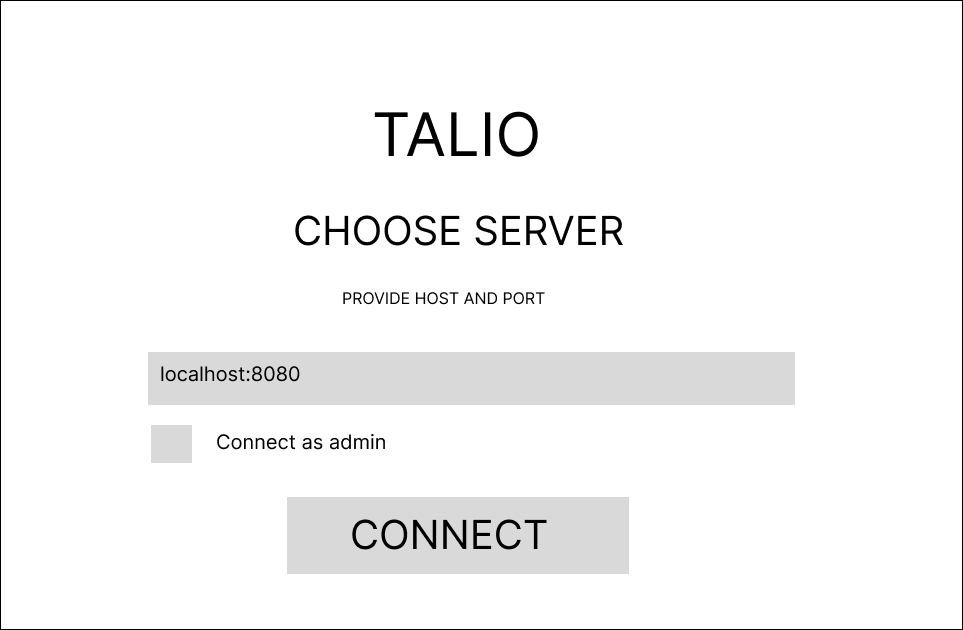
\includegraphics[width=0.5\textwidth]{choose-server}
\end{figure}

\begin{figure}[H]
\caption{If the combination of password and server is correct the admin is connected. Else a red border appears on those fields. The admin has the same client but all boards existent on the server are shown and there are no modification restrictions}
\centering
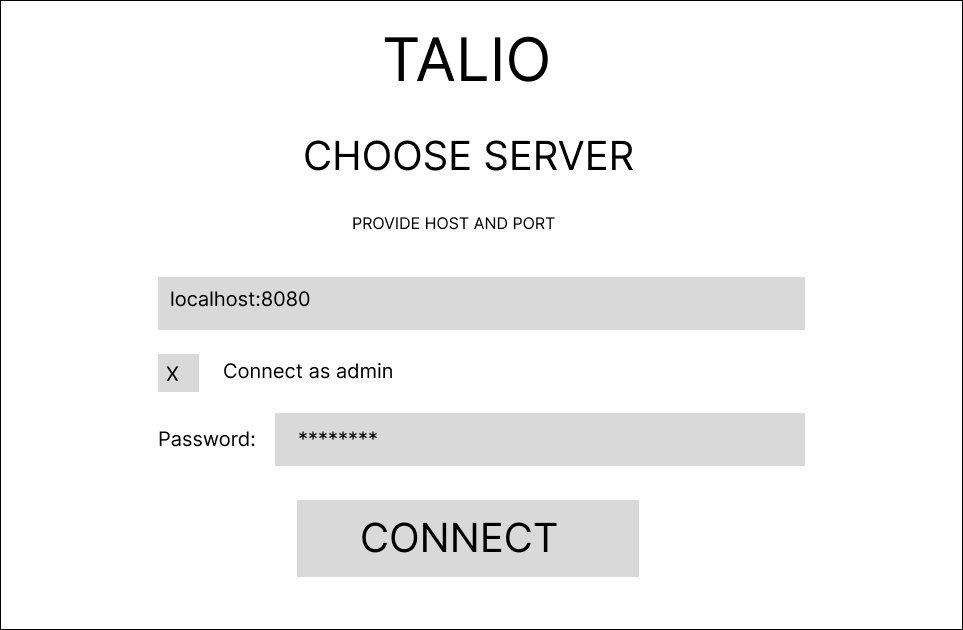
\includegraphics[width=0.5\textwidth]{choose-server-with-password}
\end{figure}

\begin{figure}[H]
\caption{This is the main page. The default board is loaded first. To share the board click on the top right button to get the sharing code. To delete the current board click the top left button. To change title click on the title on the title bar and modify it. All joined or created boards are on the left bar. Change boards by clicking on their name. To add a board click the add board button and a popup will appear. This will give you options to join an existing board by id or create a new one}
\centering
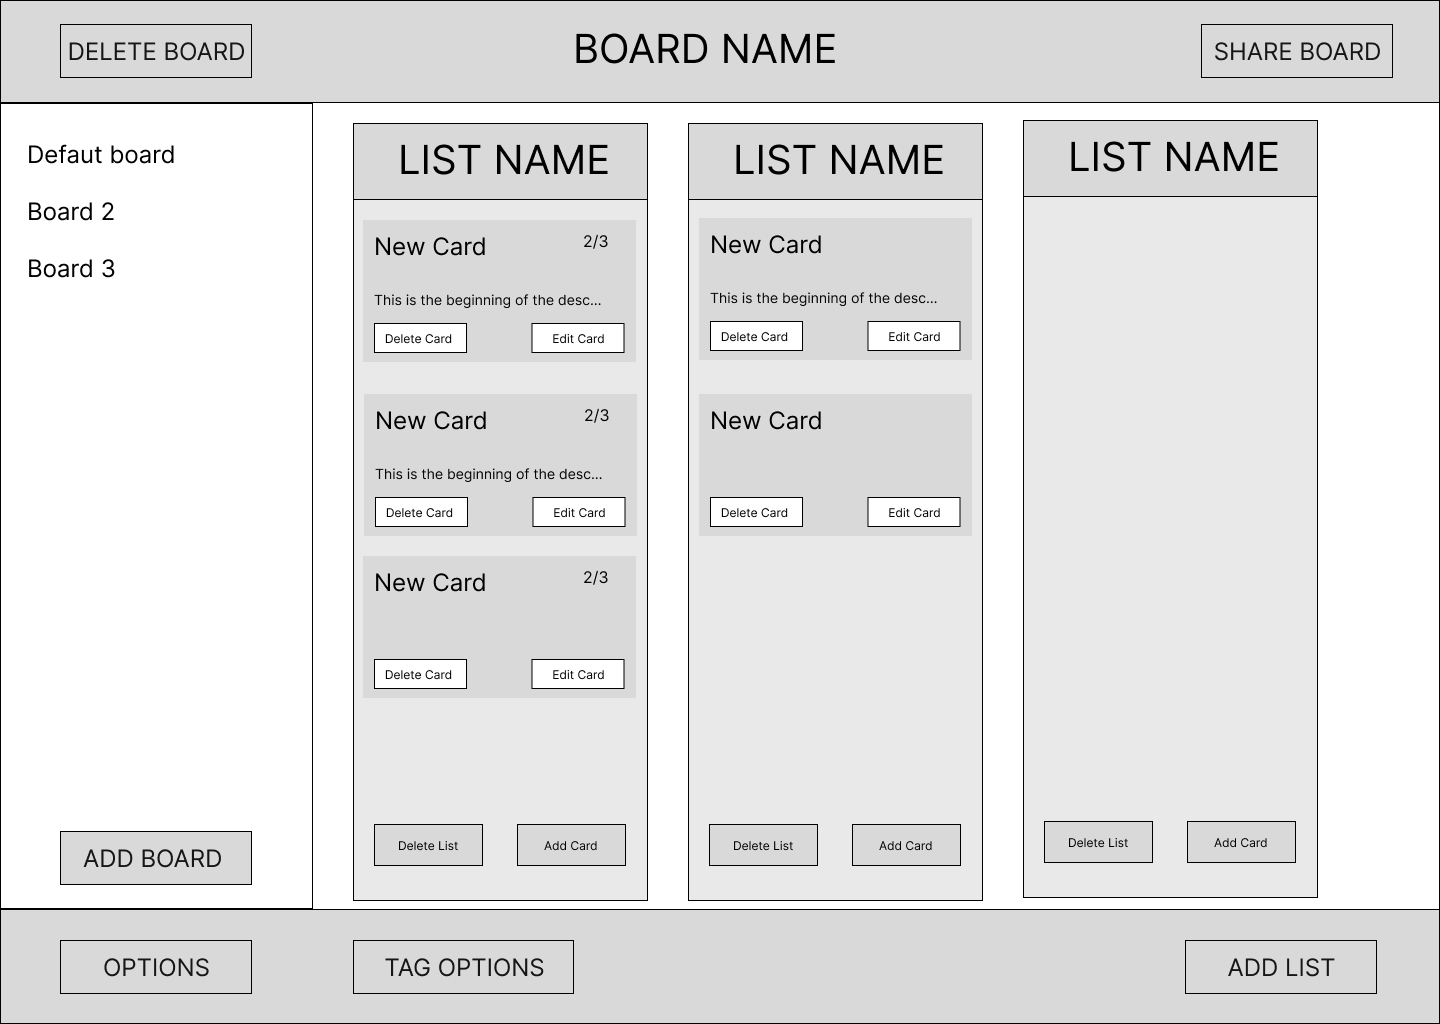
\includegraphics[width=0.5\textwidth]{main-page-1}
\end{figure}

\begin{figure}[H]
\caption{The main page after share board is clicked. The bar on the top disappears is button is clicked again or board is changed.}
\centering
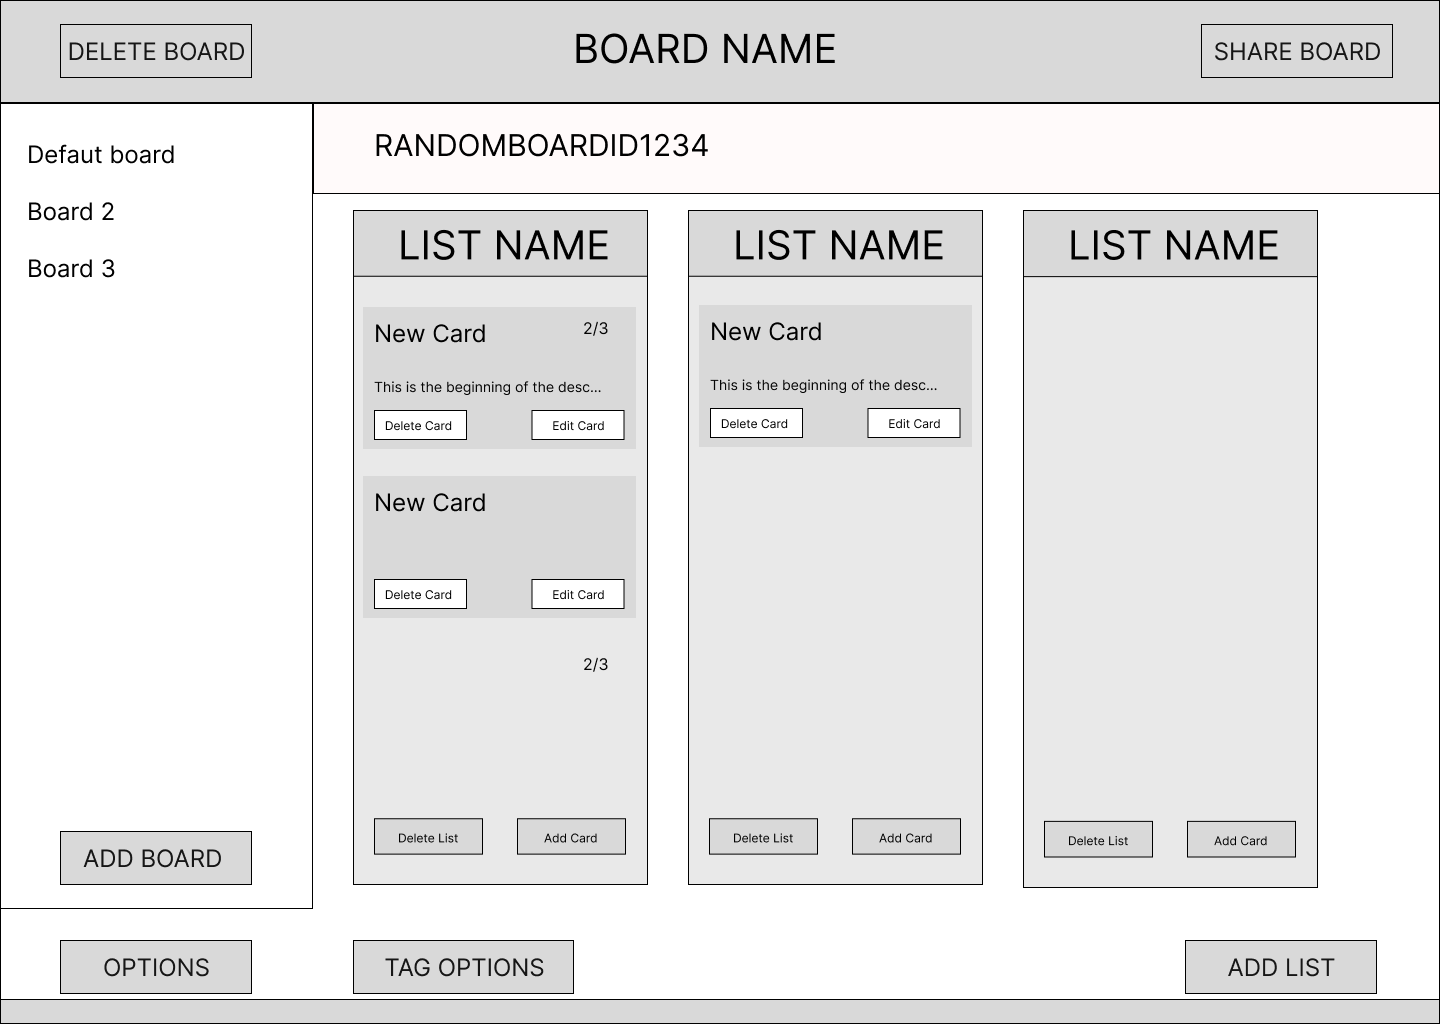
\includegraphics[width=0.5\textwidth]{main-page-5}
\end{figure}

\begin{figure}[H]
\caption{Board add pop-up}
\centering
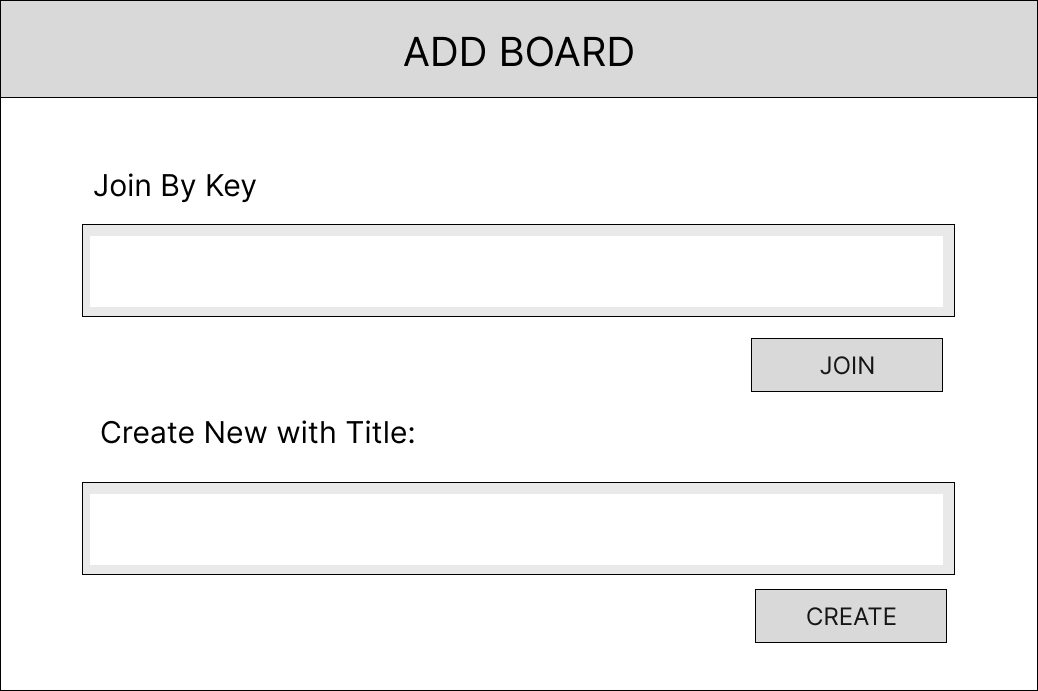
\includegraphics[width=0.5\textwidth]{board-add}
\end{figure}

\begin{figure}[H]
\caption{To add lists click the bottom-right button. If the lists don’t fit in the assigned space you can scroll horizontally. To change the name of a list click on its title and modify it. To delete it you have a button on the list. To add a card to a list you have a button on the list. If the cards don’t fit in the list you can scroll vertically inside the list. To add cards inside a list click on the button on the list. To delete cards you can press the button on the card. To edit cards (title, description, tasks, tags) click the button on the card. If the description or sub-tasks exists the cards adds distinctive details.}
\centering
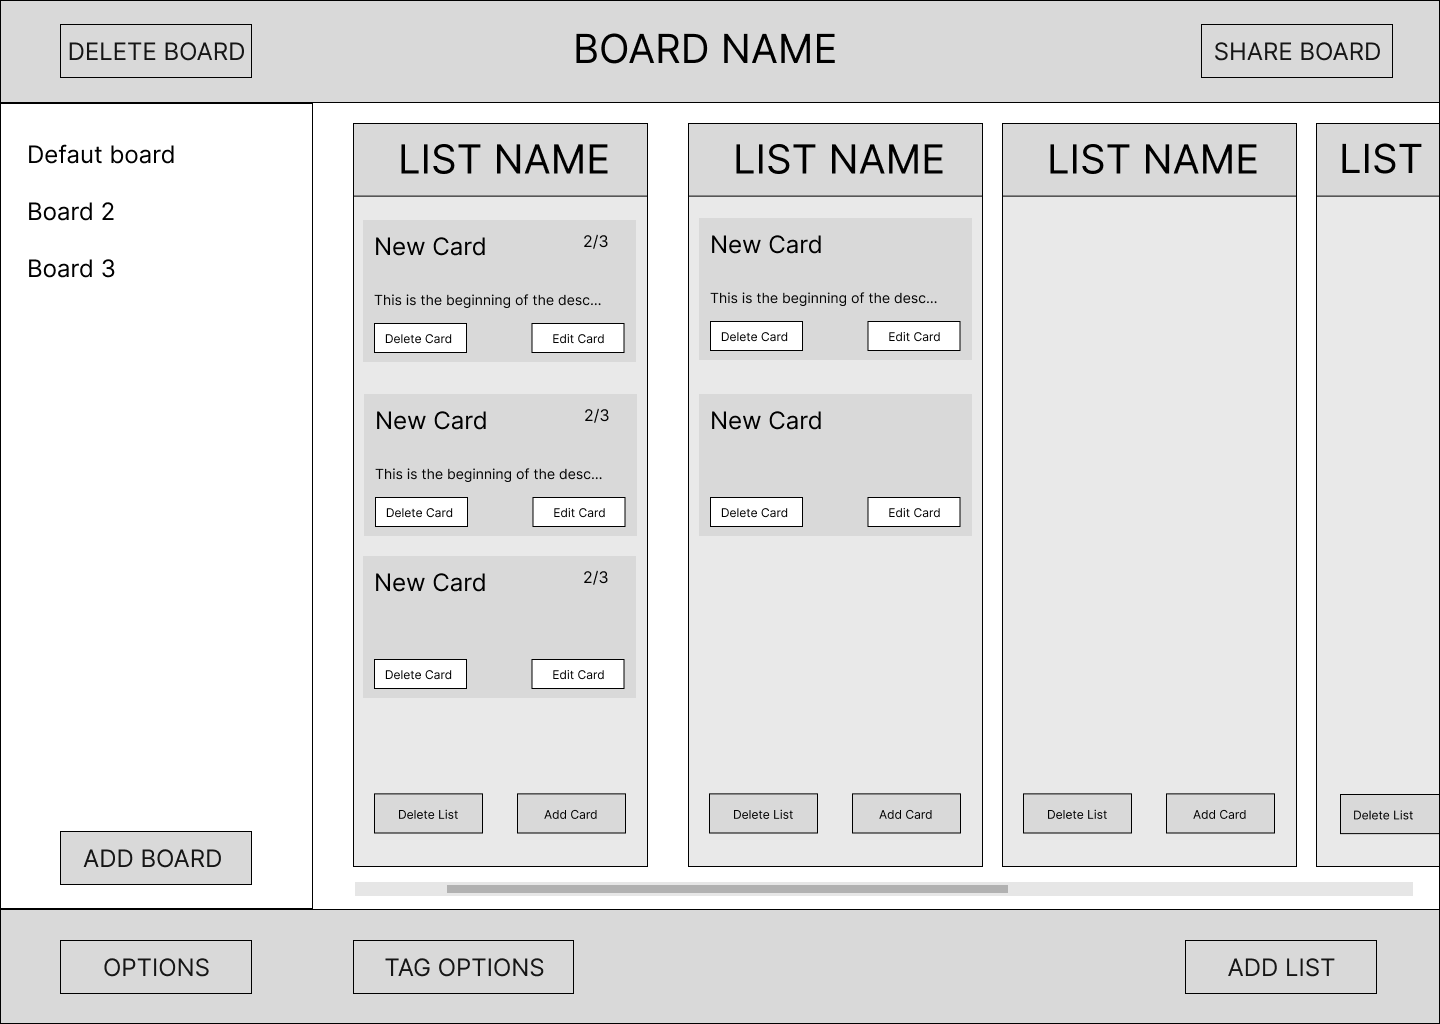
\includegraphics[width=0.5\textwidth]{main-page-2}
\end{figure}

\begin{figure}[H]
\caption{The card editing menu}
\centering
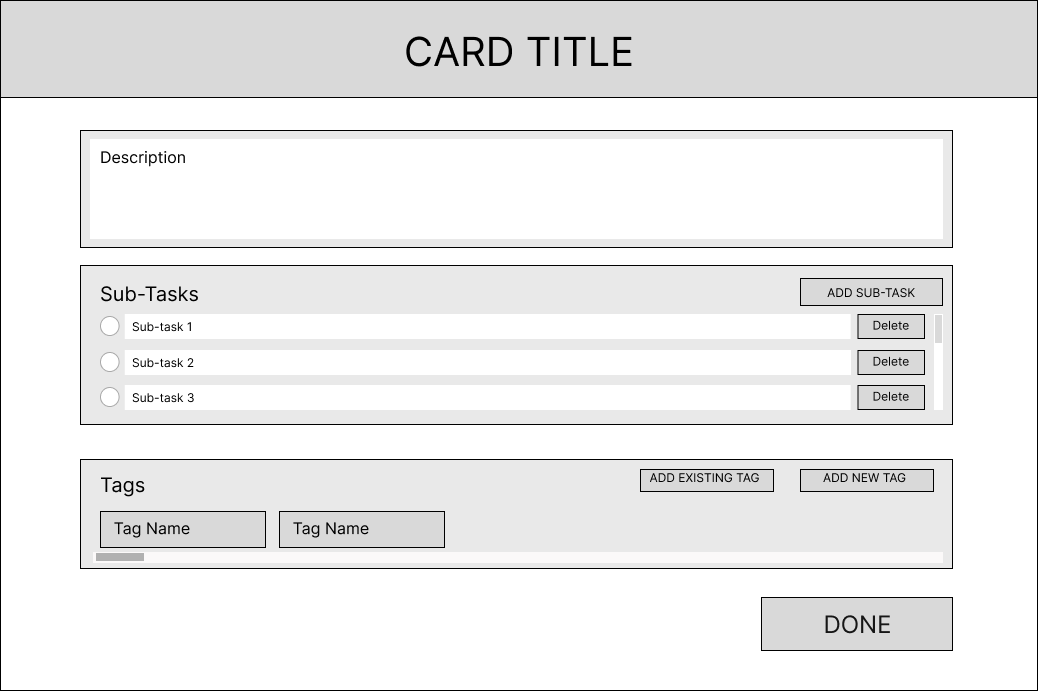
\includegraphics[width=0.5\textwidth]{edit-card}
\end{figure}

\begin{figure}[H]
\caption{The options button has a menu. Change server send you back to the first page (serve choice scene). Customization serves the customization menu. }
\centering
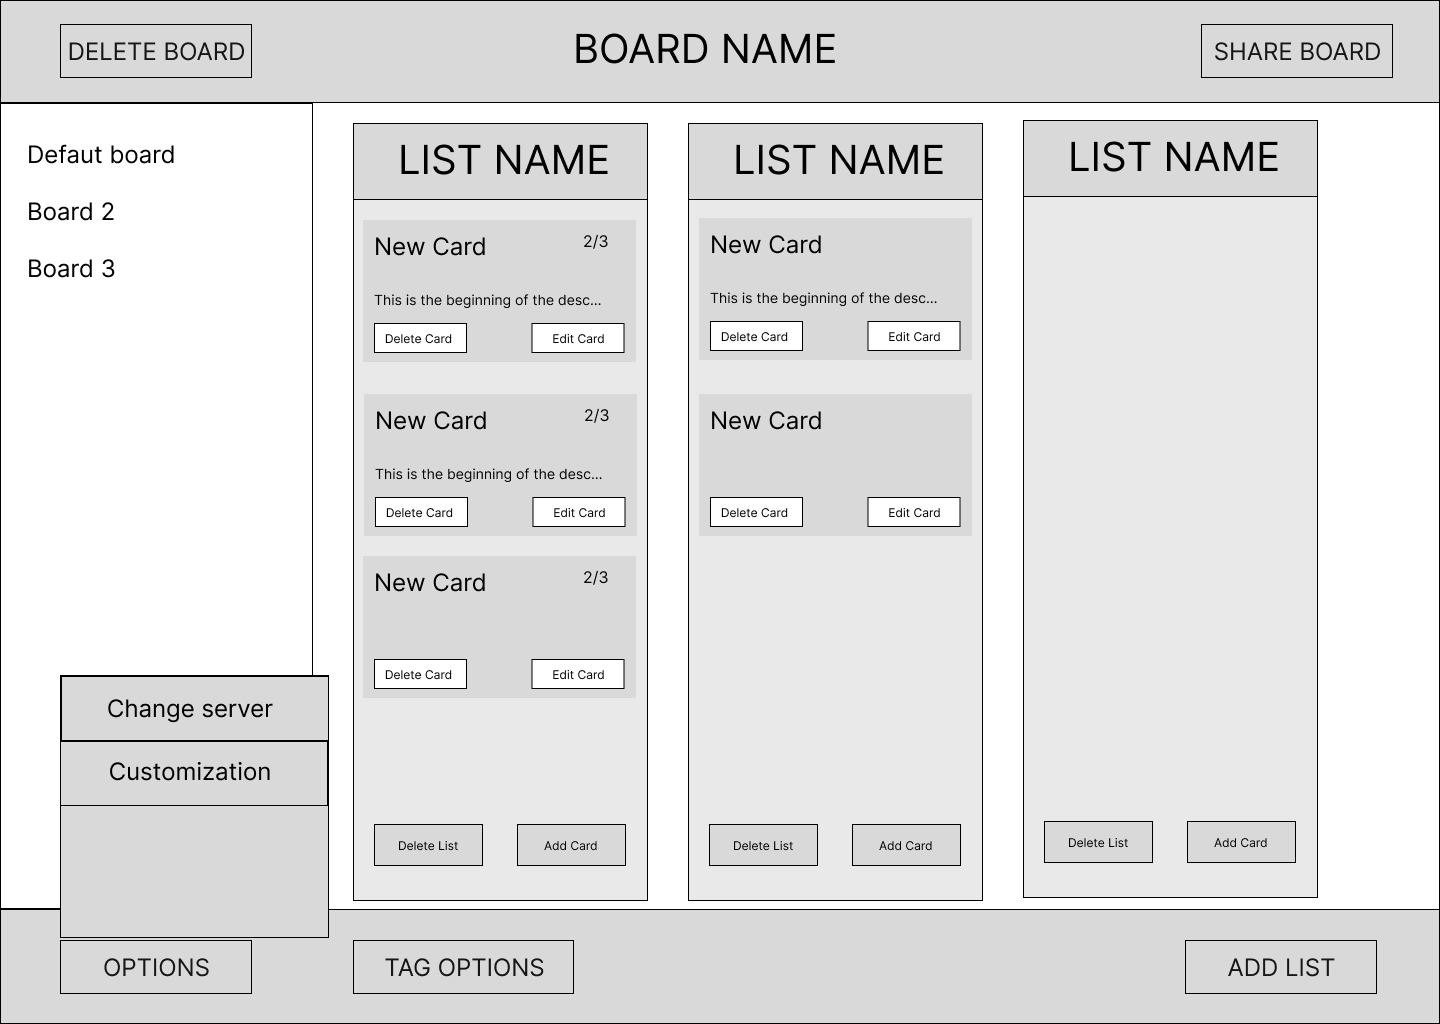
\includegraphics[width=0.5\textwidth]{main-page-3}
\end{figure}

\begin{figure}[H]
\caption{The customization menu. The user can change the background color of the board, cards or lists. The color is saved on the server and is loaded when the board is loaded.}
\centering
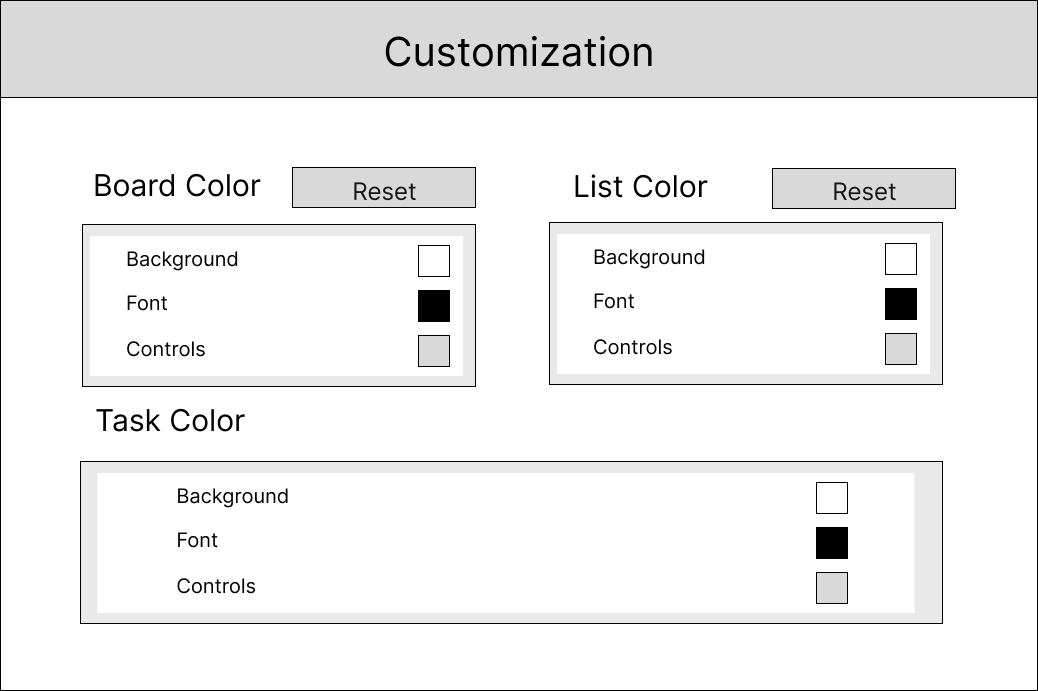
\includegraphics[width=0.5\textwidth]{customization}
\end{figure}

\begin{figure}[H]
\caption{Pressing on the colored square, leads to opening a color picker menu.}
\centering
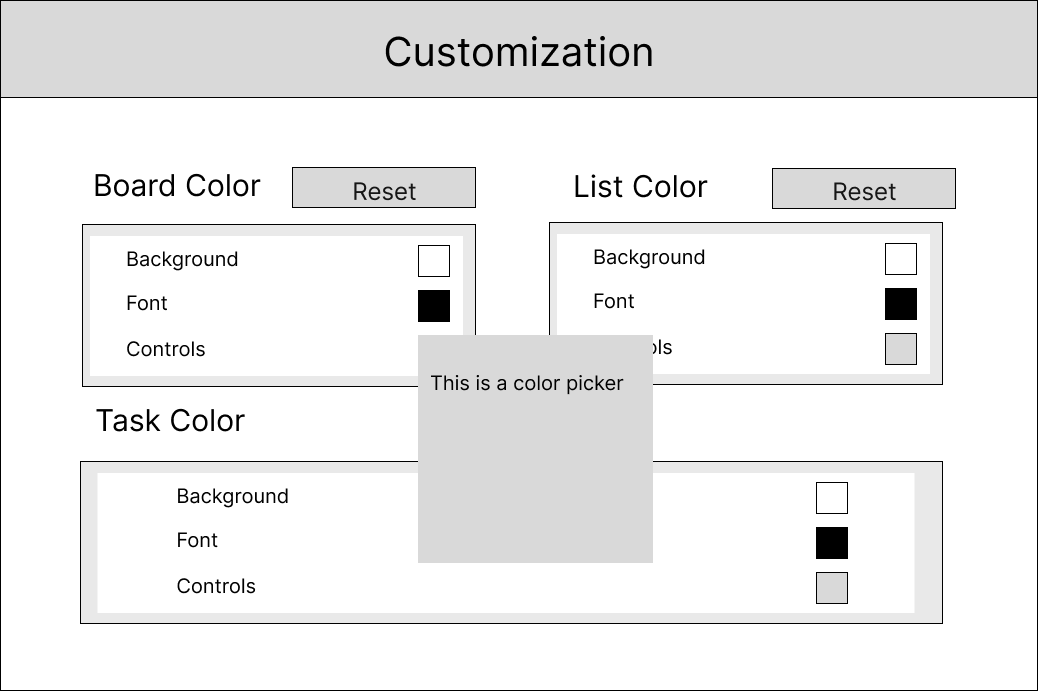
\includegraphics[width=0.5\textwidth]{color-picker}
\end{figure}

\begin{figure}[H]
\caption{If tags are selected only the cards with those tags are shown and an overview of the selected tags appears on the bottom. If no tags are selected the bar on the bottom is not shown and all cards are presented. Tag options button gives a menu for tag settings.}
\centering
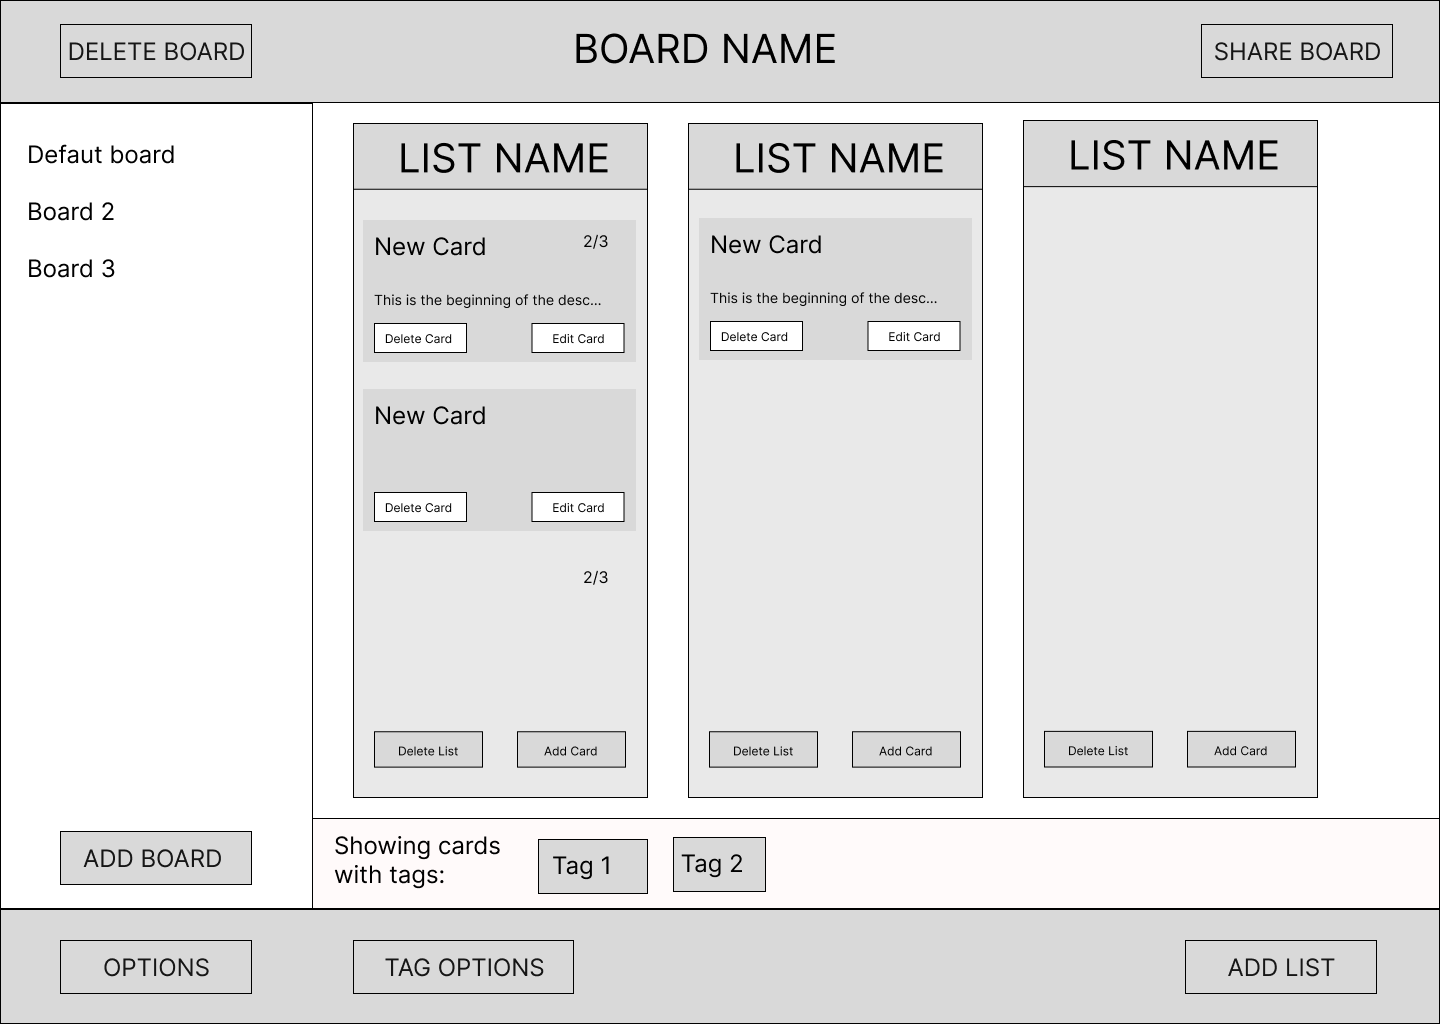
\includegraphics[width=0.5\textwidth]{main-page-4}
\end{figure}

\begin{figure}[H]
\caption{Tag options menu. This menu gives options to add, delete tags and pick which tags are allowed to be shown on the board. If no tags are selected, everything is shown.}
\centering
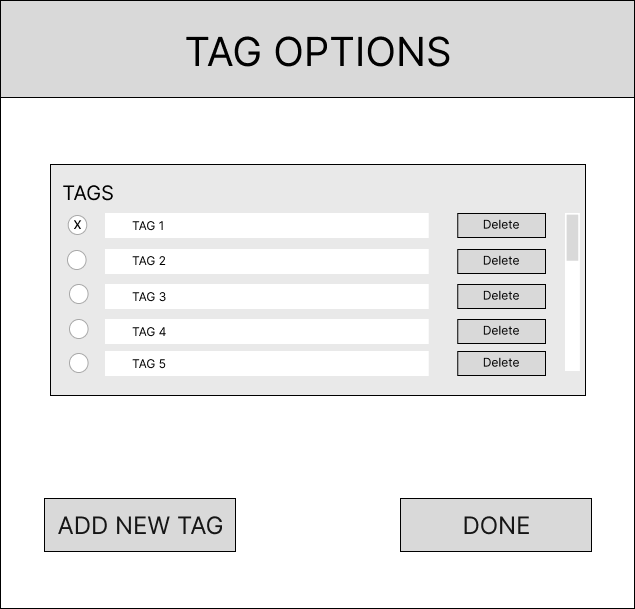
\includegraphics[width=0.5\textwidth]{tag-options}
\end{figure}

\begin{figure}[H]
\caption{Tag edit menu. This menu appears when creating a new tag. Gives options for a title and picking the colour of the tag with a color picker.}
\centering
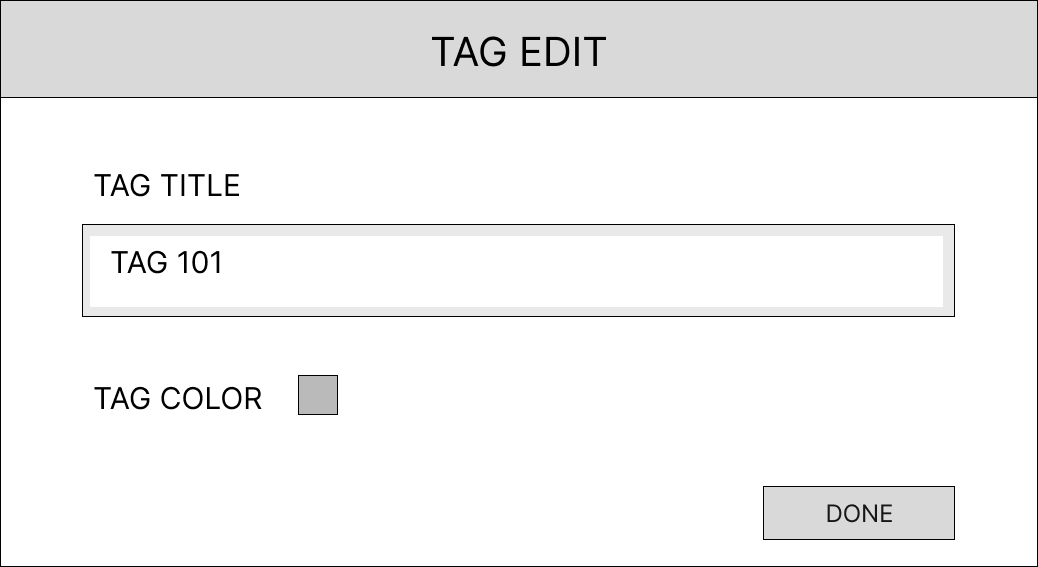
\includegraphics[width=0.5\textwidth]{tag-edit}
\end{figure}
